% --- Safety guard: define \arraybackslash if the array package failed to (e.g. broken MiKTeX install) ---
\makeatletter
\providecommand{\arraybackslash}{\let\\\@arraycr}
\makeatother
% ---------------------------------------------------------------------------------------------------
\chapter{Criterion 1: Program Educational Objectives (PEOs)}\label{criterion-1-program-educational-objectives}

Program Educational Objectives (PEOs) are the attributes and abilities that the graduates are expected to demonstrate within a few years of graduation, translated directly from the program's vision and mission and aligned with those of the University and School. Figure~\ref{fig:peo_process} gives an overview of the PEO development, evaluation, and continuous improvement process followed by the Software Engineering (SE) program at NUST-SEECS. The process incorporates input from internal stakeholders, including faculty and senior management, and external stakeholders, particularly industry representatives through the Industrial Advisory Board (IAB), while considering the requirements of relevant regulatory bodies, including PEC and HEC. PEO attainment is assessed via Alumni and Employer surveys, and the results feed into the CQI process governing subsequent revisions of PEOs, program's courses and teaching methodology.

\begin{figure}[tb]
\centering
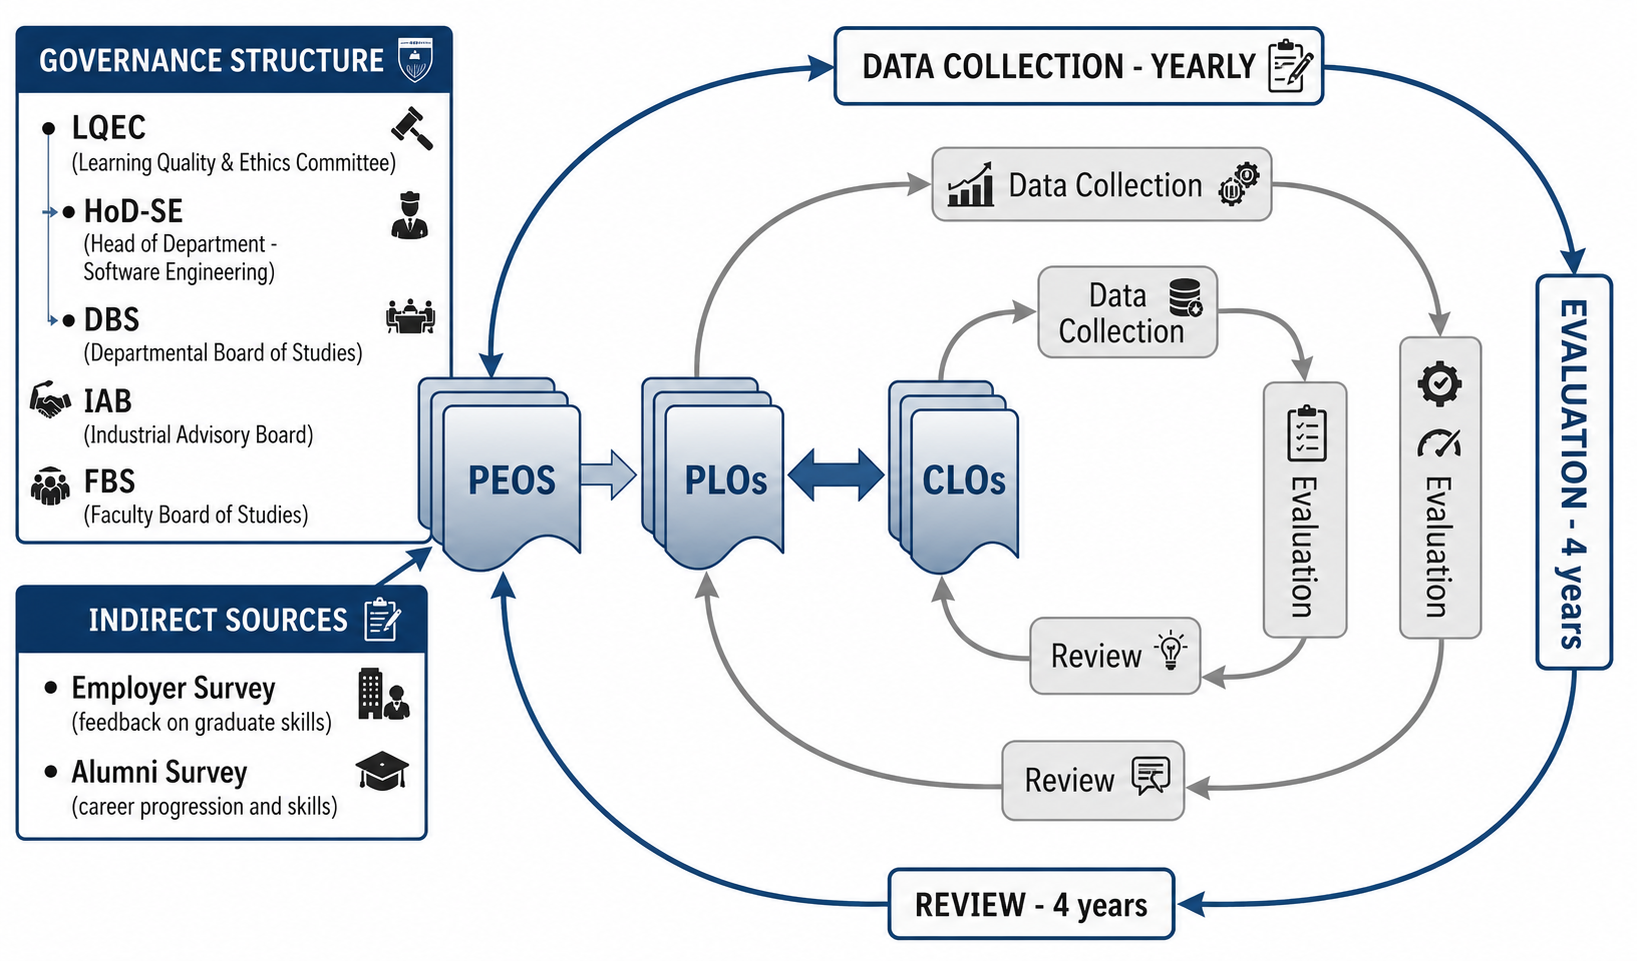
\includegraphics[width=0.9\textwidth]{images/criterion_1/media/peo-evaluation.png}
\caption{PEO Development, Evaluation, and Continuous Improvement Process}
\label{fig:peo_process}
\end{figure}

%This chapter presents the vision and mission of NUST, SEECS, and the SE Department (Section~\ref{vision-mission}), the formulation, publication, and alignment of the SE program's PEOs (Section~\ref{peo-se}), the legacy and revised (2026) PEO attainment evaluation mechanisms (Section~\ref{attainment-of-peos}) and their results (Section~\ref{attainment-results}), and how these PEO attainment results drive continuous improvement of the program supplemented by the stakeholder (industry) feedback (Section~\ref{program-improvement}).

\hypertarget{vision-mission}{%
\section{Vision \& Mission of the University, School, \& Department}\label{vision-mission}}

The vision and mission statements of NUST\footnote{https://nust.edu.pk/about-us/visionandmission/}, SEECS\footnote{https://seecs.nust.edu.pk/about-us/vision-mission/}, and the SE Department\footnote{https://seecs.nust.edu.pk/departments/department-of-software-engineering/} provide the foundational reference points against which the program's PEOs are formulated and periodically reviewed. The NUST vision and mission statements are published on the university's official website, in the university prospectus and student handbook, and on display boards across the university. The SEECS and SE Department vision and mission statements are published on their respective official websites and displayed on boards within the department. The statements are presented below in hierarchical order, from the university level to the department level.

\begin{description}[leftmargin=1.6em,style=sameline,itemsep=5pt,topsep=4pt]
\item[NUST Vision:] NUST aspires to be a comprehensive university providing a higher education experience grounded in thought leadership, co-creation of knowledge, and sustainability.
\item[NUST Mission:] NUST is committed to being a university that stimulates intellectual curiosity, behavioral progression, and environmental stewardship. We nurture future leaders, job creators, and lifelong learners, with the ability to foster partnerships, and intercultural competence to impact their communities and beyond. Through adherence to our core values, we create an ecosystem that promotes research, innovation, and productivity.
\item[SEECS Vision:] To be a center of excellence for imparting high-quality education, promoting cutting-edge research and cultivating entrepreneurial culture, while instilling sound humanitarian values thus, contributing towards the knowledge economy of Pakistan.
\item[SEECS Mission:] In pursuance to NUST's vision, SEECS strives:
\begin{itemize}[leftmargin=1.3em,nosep,topsep=3pt]
\item To provide world-class education in the fields of Electrical Engineering and Computing through dedicated faculty, continuous quality improvement and a fair and conducive environment.
\item To promote progressive research through engagement with industry, government, and international collaborators.
\item To instill the spirit of humanity through awareness of social issues and participation in co/extra-curricular activities and community service.
\item To contribute to the development and economic progress of Pakistan by promoting the culture of entrepreneurship and enhancing leadership skills.
\end{itemize}
\item[Department Vision:] To become a world class Software Engineering program, focused on quality teaching, research and entrepreneurship in order to have a positive impact on society.
\item[Department Mission:] To prepare Software Engineering graduates having a concrete knowledgebase, sound analytical skills, and professional attitude through an enabling environment to undertake real world engineering problems, innovative research, and entrepreneurship, thus contributing to the society.
\end{description}

\hypertarget{peo-se}{%
\section{PEOs: Software Engineering Program at SEECS}\label{peo-se}}

\subsection{Formulation, Improvement, and Approval of PEOs} \label{sec:peo_process} 

The Software Engineering PEOs at NUST-SEECS are formulated based on desired graduate attributes, stakeholder input, and alignment with the vision and mission of NUST, SEECS, and the SE Department. As shown in Figure~\ref{fig:peo_process}, the PEOs undergo review by the LQEC, endorsement by the Head of Department (HoD-SE), review and approval by DBS, external feedback and endorsement by the IAB, and final ratification by the FBS. Stakeholder feedback informs both the formulation and periodic review of the PEOs. The process draws on faculty reviews, IAB recommendations, and Alumni and Employer survey evidence described in Section~\ref{attainment-of-peos}. This input enables the department to assess the continuing relevance of the PEOs against graduate attributes, professional expectations, and institutional priorities. The department collects indirect assessment data from Alumni and Employer surveys annually, evaluates PEO attainment on a four-year cycle (Section~\ref{attainment-of-peos}), and reviews the PEO statements every four years against assessment evidence, stakeholder input, and the vision and mission of NUST, SEECS, and the SE Department. The review determines whether revisions are required. This periodic review cycle has not yet been completed under the current PEOs and represents the department's planned practice going forward.

\subsection{PEOs and Their Publication} \label{sec:peo_publication} The approved PEOs of the SE program are as follows: 
\begin{enumerate} 
\item \textbf{Demonstrate sound~software~engineering knowledge~and~skill set.} 
\item \textbf{Lead diverse teams and work collaboratively to develop innovative solutions. }
\item \textbf{Conduct~professional practice~for sustainable development with due consideration for~societal, ethical, and environmental aspects.} 
\end{enumerate} 
The PEOs are published on the SEECS website\footnote{https://seecs.nust.edu.pk/department-page/obe-peo-plo/} and are also available through the prospectus and departmental display materials.

\subsection{PEO Consistency with Vision, Mission, \& Stakeholder Requirements} \label{consistency-of-peos}
The PEOs are aligned with the vision and mission of NUST, SEECS, and the SE Department, as well as the requirements of key stakeholders. Table~\ref{tab:peo_mapping} maps each PEO against the applicable vision and mission statements at each institutional level. A $\checkmark$ indicates direct, substantive alignment, while $\sim$ denotes partial or indirect alignment. PEO~2, which focuses on teamwork and collaborative leadership, is marked as partially aligned where these attributes are not explicitly reflected in the relevant vision and mission statements.

%\begin{landscape}
\begingroup
\footnotesize
\setlength{\tabcolsep}{5pt}
\renewcommand{\arraystretch}{1.15}
\begin{longtable}{@{}>{\centering\arraybackslash}p{0.03\textheight} >{\raggedright\arraybackslash}p{0.10\textheight} >{\raggedright\arraybackslash}p{0.37\textheight} >{\centering\arraybackslash}p{0.020\textheight} >{\centering\arraybackslash}p{0.020\textheight} >{\centering\arraybackslash}p{0.020\textheight}@{}}
\caption{PEOs Alignment to NUST, SEECS, \& Department's Vision \& Mission. (\checkmark = strong; $\sim$ = partial).}\label{tab:peo_mapping}\\
\toprule
\textbf{S. No.} & \textbf{Vision \& Mission} & \multicolumn{1}{c}{\textbf{Description}} & \multicolumn{3}{c@{}}{\textbf{PEOs}} \\
\cmidrule(l){4-6}
 & & & \textbf{1} & \textbf{2} & \textbf{3} \\
\midrule
\endfirsthead
\toprule
\textbf{S. No.} & \textbf{Vision \& Mission} & \multicolumn{1}{c}{\textbf{Description}} & \multicolumn{3}{c@{}}{\textbf{PEOs}} \\
\cmidrule(l){4-6}
 & & & \textbf{1} & \textbf{2} & \textbf{3} \\
\midrule
\endhead
\midrule
\multicolumn{6}{r}{\footnotesize\itshape Continued on next page}\\
\endfoot
\bottomrule
\endlastfoot
1 & NUST Vision & NUST aspires to be a comprehensive university providing a higher education experience grounded in thought leadership, co-creation of knowledge, and sustainability. & \checkmark & $\sim$ & \checkmark \\
\midrule
2 & NUST Mission & NUST is committed to being a university that stimulates intellectual curiosity, behavioral progression, and environmental stewardship. We nurture future leaders, job creators, and lifelong learners, with the ability to foster partnerships, and intercultural competence to impact their communities and beyond. Through adherence to our core values, we create an ecosystem that promotes research, innovation, and productivity. & \checkmark & \checkmark & \checkmark \\
\midrule
3 & SEECS Vision & To be a center of excellence for imparting high-quality education, promoting cutting-edge research and cultivating entrepreneurial culture, while instilling sound humanitarian values thus contributing towards the knowledge economy of Pakistan. & \checkmark & $\sim$  & \checkmark \\
\midrule
4 & SEECS Mission & In pursuance to our vision, SEECS strives to:
\begin{itemize}[leftmargin=1.2em,nosep,topsep=2pt]
\item To provide world-class education in the fields of Electrical Engineering and Computing through dedicated faculty, continuous quality improvement and a fair and conducive environment.
\item To promote progressive research through engagement with industry, government, and international collaborators.
\item To instill the spirit of humanity through awareness of social issues and participation in co/extra-curricular activities and community service.
\item To contribute in the development and economic progress of Pakistan by promoting the culture of entrepreneurship and enhancing leadership skills.
\end{itemize} & \checkmark & \checkmark & \checkmark \\
\midrule
5 & SE Vision & To become a world class Software Engineering institute, focused on quality teaching, research and entrepreneurship in order to have a positive impact on society. & \checkmark & $\sim$ & \checkmark \\
6 & SE Mission & To prepare Software Engineering graduates having a concrete knowledgebase, sound analytical skills, and professional attitude through an enabling environment to undertake real world engineering problems, innovative research, and entrepreneurship, thus contributing to the society. & \checkmark & $\sim$ & \checkmark \\
\bottomrule
\end{longtable}
\endgroup
%\end{landscape}

Each PEO is supported by specific program provisions and reflects stakeholder priorities identified through faculty reviews, IAB sessions, and PEC/HEC guidelines. PEO 1, focusing on software engineering knowledge and skills, is supported by qualified faculty, laboratory facilities, and a PEC-compliant student–faculty ratio, addressing industry expectations for technical currency and PEC’s Washington Accord requirements for engineering knowledge and complex problem-solving. PEO 2, emphasizing collaborative leadership and innovation, is supported through curriculum-embedded teamwork and communication activities, oral presentations across courses, mock interviews for final-year students, a dedicated Entrepreneurship course, and industry-linked projects through the ILO. These provisions address industry recommendations on teamwork, communication, and customer orientation raised during multiple IAB sessions. PEO 3, focusing on ethical professional practice and sustainable development, reflects PEC/HEC expectations for professional ethics and regulatory compliance, alongside industry emphasis on ethical, techno-commercial professionalism raised during IAB discussions. It is supported through professional ethics coursework, industry guest lectures, mandatory UN SDG alignment in FYDPs, and a dedicated Community Service Learning course. Alumni and employer surveys, together with stakeholder feedback and attainment results, inform the evaluation of PEO relevance and identification of improvement opportunities.

%Beyond this formulation and approval process, the department intends to operate a periodic mechanism for reviewing and, where warranted, revising the PEO statements themselves (Figure~\ref{fig:peo_process}): indirect-source data from the Alumni and Employer surveys would be collected yearly, feeding into a formal evaluation of PEO attainment on a four-year cycle (Section~\ref{attainment-of-peos}), with a corresponding four-yearly review of the PEO statements against this evidence, stakeholder input, and the vision and mission of NUST, SEECS, and the department, to determine whether the PEOs require revision. This cadence has not yet completed a full cycle under the current PEOs and represents the department's planned practice going forward rather than a completed review.

\hypertarget{attainment-of-peos}{%
\section{Processes to Evaluate the Attainment of PEOs}\label{attainment-of-peos}}
PEO attainment itself is evaluated using indirect Alumni and Employer surveys.  A legacy evaluation system was used in preceding years, and a revised evaluation system was introduced in 2026 to address the legacy system's limitations. Results for both are presented in Section~\ref{attainment-results}.

\subsection{Legacy Evaluation System (till 2025)}

The legacy evaluation system used an Alumni Survey (9 items) and an Employer Survey (7 items), rated on a five-point scale (Excellent to Poor), except for four Alumni items recorded as binary Yes/No responses. Under this system, each PEO was assessed through a set of KPIs derived from these surveys, with an attainment threshold of 50\% or 60\% depending on the indicator. A PEO was considered attained only if \emph{all} of its constituent sub-KPIs individually met their respective thresholds, with cumulative PEO attainment computed as the equal-weight average of its sub-KPIs. The full survey forms are provided in Annexure~\ref{app:legacy forms} and the detailed evaluation mechanism is reported in Annexure~\ref{app:legacy_peo_evaluation}.

\subsection{Revised Evaluation System (2026)}

The transition to the revised evaluation system was motivated by two independent findings, (i) a lack of correlation between certain PEO-2/PEO-3 sub-KPI survey items, noted during the previous PEC accreditation visit and (ii) a concern raised by IAB Board members at the 13th November 2023 meeting that item 5 of the legacy Alumni Survey did not adequately assess PEO-2 attainment (see Annexure~\ref{app:iab_feedback_full}). Together, these findings led to a full redesign of the Alumni and Employer Survey instruments, mapping each item directly to a PEO. The revised forms were reviewed and formally approved by the DBS on 20th April 2026, with a decision to forward them to the FBS for final approval (Annexure~\ref{app:governance_minutes}). Later, these were presented and ratified by the FBS on 21st April 2026, and finally endorsed by the IAB on 5th May 2026. The IAB-endorsed version of the forms (Annexure~\ref{app:revised forms}) was then administered to Alumni and Employers by email and at the department's Open House in May 2026 to collect the response data reported in this section.

\subsubsection{Survey Instruments}

For the 2026 cycle, revised Alumni and Employer survey instruments replace the loosely-correlated legacy items identified above, improving alignment with PEO-level outcomes, indicator clarity, and measurability. Each survey comprises twelve items on a five-point Likert scale (Strongly Disagree to Strongly Agree), with four items mapped directly to each PEO (the full item text of both forms is presented in Annexure~\ref{app:revised forms}). Thematically, the items span across all three PEOs. For PEO~1, SE knowledge, core practices (requirements, design, coding, testing, tooling), quality attributes (performance, security), and skill currency are covered. For PEO~2, leadership, cross-functional collaboration, idea contribution, and communication with technical and non-technical audiences are covered. Finally, for PEO~3, ethical/regulatory compliance, sustainability-conscious decisions, societal/environmental impact, and professionalism are covered. Alumni and Employer items mirror each other as self- versus observer-assessments of the same indicator.

\subsubsection{Evaluation Mechanism}

The revised system evaluates each PEO indirectly through four Alumni Survey indicators and four Employer Survey indicators. For this assessment cycle, all eight indicators are assigned equal weights (0.25) to keep the scheme simple, transparent, and objective. Differentiated weighting may be introduced in later cycles through the Continuous Quality Improvement (CQI) process.

\paragraph{Question-Level KPI (QL-KPI):}
For each survey question, a Question-Level KPI (QL-KPI) is computed as the mean score of all valid responses:

\begin{equation}
Q_i=\frac{\sum_{k=1}^{n} x_k}{n}
\end{equation}

where $x_k$ represents the response of participant $k$ and $n$ is the total number of valid responses (excluding N/A entries). Responses are recorded on a five-point Likert scale coded from 0 to 4 (0 = Strongly Disagree, 1 = Disagree, 2 = Neutral, 3 = Agree, 4 = Strongly Agree). A score of \textbf{2.0 or above} (i.e., Neutral or better) is considered acceptable performance at the indicator level.

\paragraph{Stakeholder-Level PEO Score:}
For each PEO, the four Alumni indicators and the four Employer indicators are aggregated separately using equal weights:

\begin{equation}
PEO_{Alumni}=0.25Q_1+0.25Q_2+0.25Q_3+0.25Q_4
\end{equation}

\begin{equation}
PEO_{Employer}=0.25Q_1+0.25Q_2+0.25Q_3+0.25Q_4
\end{equation}

\paragraph{Stakeholder Integration:}
The overall PEO score combines the Alumni and Employer assessments with equal contribution:

\begin{equation}
PEO_{Score}=0.5(PEO_{Alumni})+0.5(PEO_{Employer})
\end{equation}

This ensures balanced consideration of both graduate self-assessment and employer evaluation.

\paragraph{Multi-Step PEO Attainment Evaluation:}
To avoid misleading conclusions that may arise from simple averaging, a multi-step attainment evaluation mechanism is employed.

\textbf{Step 1 - Indicator Evaluation:} Each question mapped to a PEO is evaluated independently against the Question-Level KPI threshold:

\begin{equation}
QL\text{-}KPI \geq 2.0
\end{equation}

\textbf{Step 2 - Indicator Coverage Requirement:} At least three out of four indicators associated with a PEO must satisfy the Question-Level KPI threshold:

\begin{equation}
\text{Coverage Requirement} = \frac{\text{Indicators Meeting Threshold}}{\text{Total Indicators}}
\geq 75\%
\end{equation}

This ensures that attainment is consistently demonstrated across multiple dimensions and is not driven by isolated strengths.

\textbf{Step 3 - PEO-Level Evaluation:} The aggregated PEO score is normalized to a 0--1 scale. Because responses are coded on a 0--4 scale, the normalization divides by the scale maximum:

\begin{equation}
PEO_{Normalized}=
\frac{PEO_{Score}}{4}
\end{equation}

A PEO is considered attained if:

\begin{equation}
PEO_{Normalized}\geq0.60
\end{equation}

The normalized score is interpreted according to Table~\ref{tab:peo_interpretation}.

\begin{table}[htbp]
\centering
\caption{PEO Attainment Interpretation}
\begin{tabular}{|c|c|}
\hline
\textbf{Normalized Score} & \textbf{Attainment Status} \\
\hline
$\geq 0.60$ & Attained \\
\hline
0.50 -- 0.59 & Partially Attained \\
\hline
$<0.50$ & Not Attained \\
\hline
\end{tabular}
\label{tab:peo_interpretation}
\end{table}

The revised framework establishes a clear traceability path from survey responses to indicators, to stakeholder scores, and finally to PEO attainment, forming the basis for periodic review and CQI.

\hypertarget{attainment-results}{%}
\section{PEO Attainment Results}\label{attainment-results}}

\subsection{Legacy Evaluation Results (2025)}

Using 2025 Alumni and Employer survey data and the legacy criterion requiring every sub-KPI to meet its threshold, PEO~2 and PEO~3 were fully attained. For PEO~1, five of six sub-KPIs met their thresholds, while the higher-education indicator reached 36\% against the 50\% threshold. Equal-weight cumulative attainment was approximately 75\%, 79\%, and 70\% for PEO~1, PEO~2, and PEO~3, respectively. The shortfall reflects limitations of the legacy instrument and its all-or-nothing pass rule, as pursuing higher education alone does not determine PEO attainment. Graduates entering employment are not necessarily deficient against the objective. These limitations motivated the revised evaluation system. Detailed results are provided in Annexure~\ref{app:legacy_peo_evaluation}.

\subsection{Revised Evaluation Results (2026)}

The revised assessment framework was piloted using Alumni and Employer survey data collected in 2026. A total of 79 Alumni responses and 50 Employer responses were received, with per-question valid-response counts ranging from 77--79 (Alumni) and 49--50 (Employer) owing to occasional not-applicable or blank entries. Table~\ref{tab:peo_indicators_2026} presents the indicator-level Question-Level KPI (QL-KPI) scores for each PEO, disaggregated by stakeholder group, together with the indicator coverage outcome and the stakeholder-level PEO scores. All scores are reported on the 0--4 response scale.

\begin{table}[htbp]
\centering
\caption{Indicator-Level and Stakeholder-Level Results, 2026 Assessment Cycle (0--4 scale)}
\begin{tabular}{|c|c|c|c|c|c|c|c|}
\hline
\textbf{PEO} & \textbf{Stakeholder} & \textbf{Q1} & \textbf{Q2} & \textbf{Q3} & \textbf{Q4} & \textbf{Coverage} & \textbf{Score} \\
\hline
\multirow{2}{*}{PEO 1} & Alumni & 2.91 & 3.06 & 3.25 & 3.35 & 4/4 & 3.142 \\
\cline{2-8}
 & Employer & 3.33 & 3.30 & 3.14 & 3.36 & 4/4 & 3.282 \\
\hline
\multirow{2}{*}{PEO 2} & Alumni & 3.37 & 3.30 & 3.36 & 3.28 & 4/4 & 3.327 \\
\cline{2-8}
 & Employer & 3.22 & 2.98 & 3.02 & 3.00 & 4/4 & 3.055 \\
\hline
\multirow{2}{*}{PEO 3} & Alumni & 3.35 & 3.13 & 3.13 & 3.49 & 4/4 & 3.275 \\
\cline{2-8}
 & Employer & 3.18 & 3.10 & 3.14 & 3.18 & 4/4 & 3.150 \\
\hline
\end{tabular}
\label{tab:peo_indicators_2026}
\end{table}

For every PEO, all four indicators from both stakeholder groups met the QL-KPI threshold of 2.0, satisfying the indicator coverage requirement of at least three out of four indicators. The stakeholder-level scores were then combined using equal weighting and normalized to the 0--1 scale. Table~\ref{tab:peo_attainment_2026} summarizes the final PEO attainment outcomes.

\begin{table}[htbp]
\centering
\caption{PEO Attainment Summary, 2026 Assessment Cycle}
\begin{tabular}{|c|c|c|c|}
\hline
\textbf{PEO} & \textbf{Aggregated Score $S$ (0--4)} & \textbf{Normalized Score $S/4$} & \textbf{Status} \\
\hline
PEO 1 & 3.212 & 0.803 & Attained \\
\hline
PEO 2 & 3.191 & 0.797 & Attained \\
\hline
PEO 3 & 3.212 & 0.803 & Attained \\
\hline
\end{tabular}
\label{tab:peo_attainment_2026}
\end{table}

All three PEOs achieved normalized scores above the attainment threshold of 0.60 and are therefore classified as \textbf{Attained} for the 2026 assessment cycle. Across the combined 948 Alumni responses (12 questions $\times$ 79 respondents) and 600 Employer responses (12 questions $\times$ 50 respondents), the overwhelming majority of ratings were favourable. 87.9\% of Alumni responses were ``Agree'' or ``Strongly Agree'' (359 and 474 respectively, against 84 Neutral, 14 Disagree, 5 Strongly Disagree, and 12 not-applicable/blank), and 83.3\% of Employer responses were ``Agree'' or ``Strongly Agree'' (270 and 230 respectively, against 73 Neutral, 9 Disagree, 14 Strongly Disagree, and 4 not-applicable/blank).


\hypertarget{program-improvement}{%
\section{Evaluation Results \& Continuous Program Improvement}\label{program-improvement}}

The department uses PEO attainment results, IAB recommendations, and PEC observations to identify improvement priorities and determine appropriate actions. These inputs provide complementary evidence. Attainment results inform the evaluation of graduate outcomes, while industry feedback identifies curriculum, teaching, and professional-development needs.

Of the sixteen sub-KPIs evaluated under the legacy system (Section~\ref{attainment-results}), fifteen met their attainment thresholds. The only failing indicator was PEO~1's measure of alumni pursuing higher education (36\% against a 50\% threshold). This result may reflect survey reach and career choices rather than graduate capability. Alumni who have moved abroad may be harder to contact, while others may pursue industry or entrepreneurship instead of further study. PEO~3's measure of UN SDG incorporation into graduates' work passed by only two percentage points (52\% against 50\%), the narrowest margin among the passing indicators. Its focus on academic project work also raises questions about its relevance to the professional practice of working graduates. Together with survey-item correlation weaknesses identified during the 2023 PEC accreditation visit and by the IAB (Section~\ref{attainment-of-peos}), these findings indicated that some legacy survey items were poorly aligned with the PEOs they were intended to measure. The department therefore prioritised redesigning the measurement instrument rather than changing the curriculum or teaching methodology, as the legacy results did not provide sufficient evidence to justify such changes. The IAB endorsed the revised Alumni and Employer survey instruments in 2026. In the first assessment cycle, all three PEOs achieved normalized scores above the 0.60 attainment threshold (Table~\ref{tab:peo_attainment_2026}). These results provide an initial baseline under the revised instrument but do not, by themselves, establish improved program effectiveness. The DBS will use subsequent cycles to assess indicator reliability and coverage, consider whether the attainment threshold or indicator-coverage rule should be strengthened, and refine survey items where necessary. Further curriculum or teaching changes will be guided by the resulting evidence.

The department also uses qualitative industry feedback and PEC observations to identify and track improvement actions. Table~\ref{tab:iab_meetings} summarises the four IAB sessions held since 2024. Their minutes and the recommendation-level implementation record are provided in Annexures~\ref{app:iab_minutes} and~\ref{app:iab_feedback_full}, respectively. Three earlier IAB sessions, held on 24 May, 4 July, and 13 November 2023, also informed departmental practice, including the PEO-2/PEO-3 survey redesign discussed in Section~\ref{attainment-of-peos}. These sessions are outside the 2024-onward record. 

\begin{table}[htbp] 
\centering 
\caption{IAB Meetings Held Since 2024} 

\begin{tabular}{|c|l|p{0.58\textwidth}|} \hline \textbf{S. No.} & \textbf{Date} & \textbf{Key Focus} \\ 
\hline 
1 & 2nd May 2024 & Review of curriculum changes made in response to 2023 IAB feedback: VR/AR elective, Fundamentals of Computer Programming credit-hour increase, FYDP patenting \\ 
\hline 
2 & 28th February 2025 & New elective proposals (Introduction to Quantum Computing), certification-style courses, open-book examinations, cross-departmental minors \\ \hline 
3 & 7th May 2025 & Faculty industry-alignment boot camp, splitting Applied AI/DevOps/Machine Learning course content, mentorship and cloud-resource access for students \\ 
\hline 
4 & 5th May 2026 & Endorsement of the revised (2026) Alumni and Employer survey instruments \\ 
\hline 
\end{tabular} 
\label{tab:iab_meetings} 
\end{table} 

Across these four IAB sessions, eleven recommendations and PEC observations were recorded. Four have documented implementation progress, all originating at the 28 February 2025 meeting, i.e. introduction of new electives, enablement of cross-departmental minor courses, adoption of open-book examinations, and consideration of certification-style courses. %For certifications, NUST approved an implementation mechanism recognising 1--3 credit hours for departmentally validated certifications through Working Paper No. 2, 73rd ACM,\footnote{Working Paper No. 2, 73rd ACM, 9th February 2026} endorsed at UCAP on 30 January 2026 and consistent with HEC's CS/IT-specific advisory.\footnote{Letter HEC/CURR/GEN/2025/8036, 15th September 2025} Full closure awaits PEC's final SOP, pending ratification by its Engineering Accreditation Board (EAB) and Governing Body following the PEC Task Force's proposal of a broader 6--12 credit-hour range.\footnote{Letter PEC/EAD/EQEEP/2025/04, 14th July 2025} Further details are provided in Annexure~\ref{app:certifications}. 
The remaining seven recommendations, raised at the IAB meetings of 2 May 2024, 28 February 2025, and 7 May 2025, remain open and actively tracked. They address curriculum breadth, faculty capacity-building, industry mentorship, infrastructure access, and graduate soft skills and ethics. Their implementation status is monitored to identify outstanding actions and determine follow-up measures. Separately, recommendations from the 2023 IAB sessions led to the introduction of a Virtual/Augmented Reality elective and an increase in the Fundamentals of Computer Programming course load from 3 to 4 credit hours. These actions, are documented in the 2 May 2024 IAB minutes (Annexure~\ref{app:iab_minutes}). 

%predate and are excluded from the 2024-onward recommendation record.

